\documentclass[border=2pt]{standalone}
\usepackage[T1]{fontenc}
\usepackage[scaled=1.0]{helvet}
\renewcommand{\familydefault}{\sfdefault}
\usepackage{sfmath}
\usepackage{amsmath}
\usepackage{xcolor}
\usepackage{tikz}
\usetikzlibrary{positioning,arrows.meta,calc,fit,backgrounds,shapes.geometric}
% palette (light fills, dark strokes: prints well in colour and greyscale)
\definecolor{ink}{HTML}{1F2933}
\definecolor{muted}{HTML}{52606D}
\definecolor{dataS}{HTML}{B7791F}\definecolor{dataF}{HTML}{FDF3E1}
\definecolor{physS}{HTML}{2F6DB5}\definecolor{physF}{HTML}{E6EFFA}
\definecolor{tranS}{HTML}{2E7D4F}\definecolor{tranF}{HTML}{E5F4EA}
\definecolor{repS}{HTML}{6B4FA8}\definecolor{repF}{HTML}{EFEAF8}
\definecolor{greyS}{HTML}{7B8794}\definecolor{greyF}{HTML}{F1F3F5}
\tikzset{
  >={Stealth[length=2.6mm,width=2mm]},
  box/.style={draw, rounded corners=2pt, line width=0.7pt, align=center, inner sep=4pt, text=ink},
  ttl/.style={font=\bfseries\small},
  arr/.style={->, line width=0.9pt, draw=ink},
  darr/.style={->, line width=0.8pt, draw=muted, dashed},
  stage/.style={draw, rounded corners=4pt, line width=0.6pt, dash pattern=on 3pt off 2pt, inner sep=7pt},
  stagelabel/.style={font=\bfseries\small, anchor=south west, inner sep=2pt},
}
\usepackage[none]{hyphenat}
\newcommand{\T}[1]{{\small\bfseries #1}\\[1pt]}

\begin{document}
\footnotesize
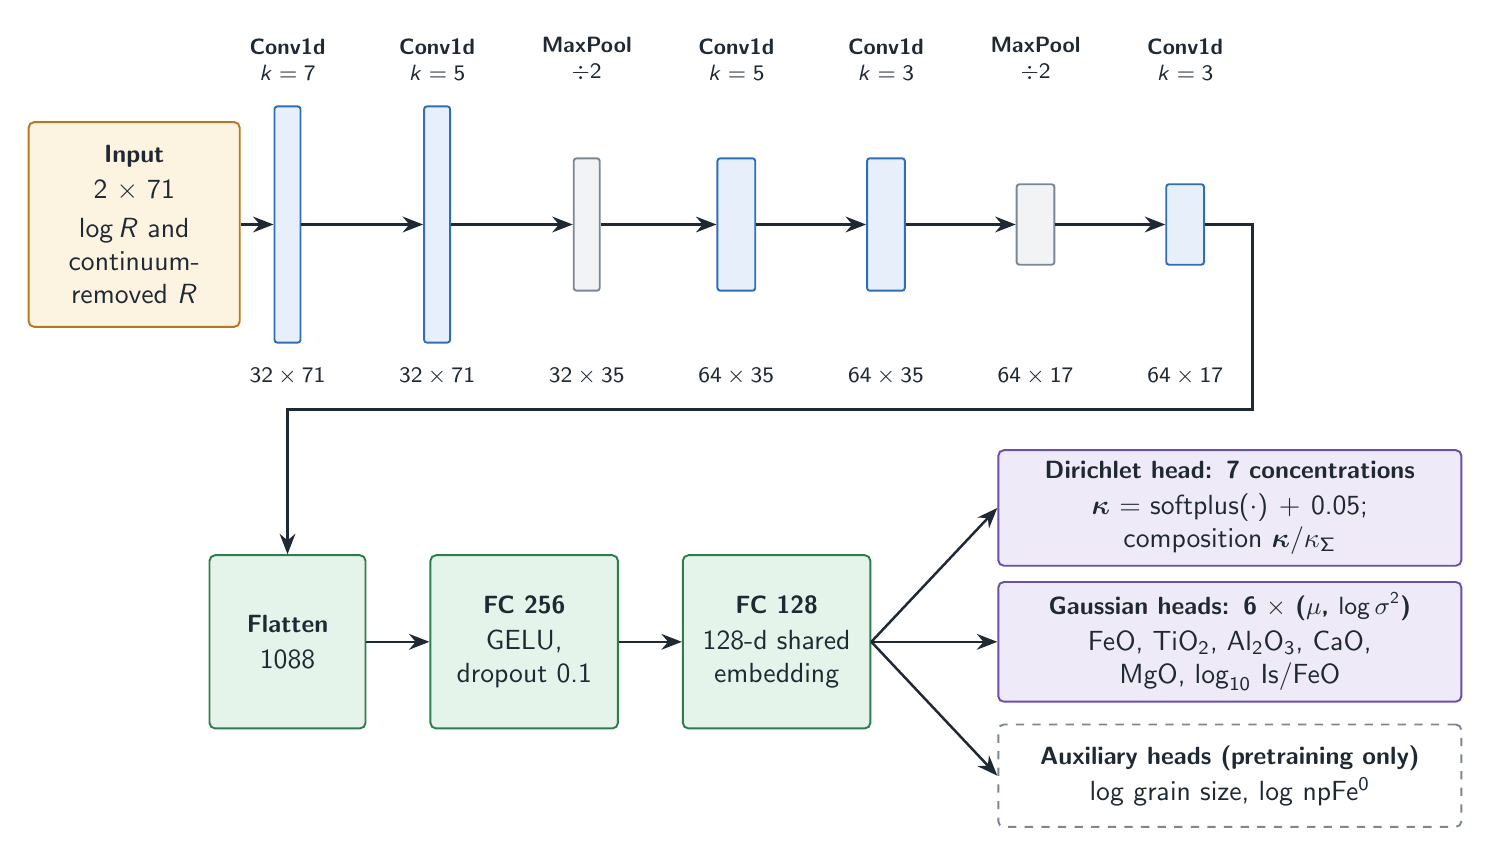
\begin{tikzpicture}
% ---------- tier 1: convolutional feature extractor ----------
\node[box, draw=dataS, fill=dataF, text width=24mm, minimum height=26mm, anchor=west] (in) at (0,0)
  {\T{Input}$2\times71$\\[2pt]$\log R$ and\\continuum-\\removed $R$};
% blocks: name, kernel/label, channels, length, type
\def\xs{33mm}
\foreach \i/\lab/\sub/\c/\l/\t in {
  1/Conv1d/{$k=7$}/32/71/c, 2/Conv1d/{$k=5$}/32/71/c, 3/MaxPool/{$\div 2$}/32/35/p,
  4/Conv1d/{$k=5$}/64/35/c, 5/Conv1d/{$k=3$}/64/35/c, 6/MaxPool/{$\div 2$}/64/17/p, 7/Conv1d/{$k=3$}/64/17/c} {
  \pgfmathsetmacro{\w}{1.8+3.0*\c/64}
  \pgfmathsetmacro{\h}{4+26*\l/71}
  \pgfmathsetmacro{\x}{33+(\i-1)*19}
  \def\cc{c}\ifx\t\cc\def\fc{physF}\def\dc{physS}\else\def\fc{greyF}\def\dc{greyS}\fi
  \node[draw=\dc, fill=\fc, line width=0.7pt, minimum width=\w mm, minimum height=\h mm, inner sep=0pt, rounded corners=1pt] (b\i) at (\x mm,0) {};
  \node[font=\footnotesize, text=ink, align=center, anchor=south] at (\x mm,17mm) {\textbf{\lab}\\\sub};
  \node[font=\footnotesize, text=ink, anchor=north] at (\x mm,-17mm) {$\c\times\l$};
}
\draw[arr] (in.east) -- (b1.west);
\foreach \a/\b in {1/2,2/3,3/4,4/5,5/6,6/7} \draw[arr] (b\a.east) -- (b\b.west);
% ---------- tier 2: shared trunk and heads ----------
\def\yy{-53mm}
\node[box, draw=tranS, fill=tranF, text width=17mm, minimum height=22mm] (fl) at (33mm,\yy) {\T{Flatten}1088};
\node[box, draw=tranS, fill=tranF, text width=21mm, minimum height=22mm, right=8mm of fl] (fc1) {\T{FC 256}GELU,\\dropout 0.1};
\node[box, draw=tranS, fill=tranF, text width=21mm, minimum height=22mm, right=8mm of fc1] (fc2) {\T{FC 128}128-d shared\\embedding};
\draw[arr] ($(b7.east)+(0,0)$) -- ++(6mm,0) |- (33mm,-23.5mm) -- (fl.north);
\draw[arr] (fl) -- (fc1); \draw[arr] (fc1) -- (fc2);
\node[box, draw=repS, fill=repF, text width=56mm, minimum height=13mm, anchor=west] (h1) at ($(fc2.east)+(16mm,17mm)$)
  {\T{Dirichlet head: 7 concentrations}$\boldsymbol\kappa$ = softplus$(\cdot)+0.05$; composition $\boldsymbol\kappa/\kappa_\Sigma$};
\node[box, draw=repS, fill=repF, text width=56mm, minimum height=13mm, anchor=west] (h2) at ($(fc2.east)+(16mm,0)$)
  {\T{Gaussian heads: 6 $\times$ ($\mu$, $\log\sigma^2$)}FeO, TiO$_2$, Al$_2$O$_3$, CaO, MgO, $\log_{10}$ Is/FeO};
\node[box, draw=greyS, fill=white, dashed, text width=56mm, minimum height=13mm, anchor=west] (h3) at ($(fc2.east)+(16mm,-17mm)$)
  {\T{Auxiliary heads (pretraining only)}$\log$ grain size, $\log$ npFe$^0$};
\foreach \h in {h1,h2,h3} \draw[arr] (fc2.east) -- (\h.west);
\end{tikzpicture}
\end{document}
